\chapter{GUI-Entwurf}
\label{chapter:gui}

Eine Software kann noch so gut geplant und durchstrukturiert sein, wenn die Benutzeroberfläche jedoch unübersichtlich ist und nicht bedient werden kann, dann ist der gesamte Rest hinfällig. Daher ist es nötig sich bereits im Vorfeld eine mögliche Front-End-Gestaltung zu überlegen. In Anbetracht der Tatsache, dass der Programmentwurf in Java umgesetzt werden wird, haben wir beim GUI-Entwurf auf die Gestaltung von zu umständlichen und modernen Bestandteilen, wie man sie heute auf den meisten Webseiten sehen kann, verzichtet und uns auf die grundlegenden Bestandteile fokussiert. 


Übergeordnet soll in der gesamten Anwendung ein einheitliches Design vorliegen. Darum haben wir uns bereits zu Beginn auf ein Farbschema abgestimmt. Basierend auf einer Mitarbeiterumfrage haben wir uns für ein rötlich-rosa Farbschema entschieden, sodass die Farben (in Hexwerten) \textbf{\#DE639A}, \textbf{\#E388B1}, \textbf{\#D7A6B3}, \textbf{\#F1E2E2}, \textbf{\#707070} ihre Anwendung fanden. 

\newpage

\section{Diagramm}

\begin{figure}[!ht]
    \centering
    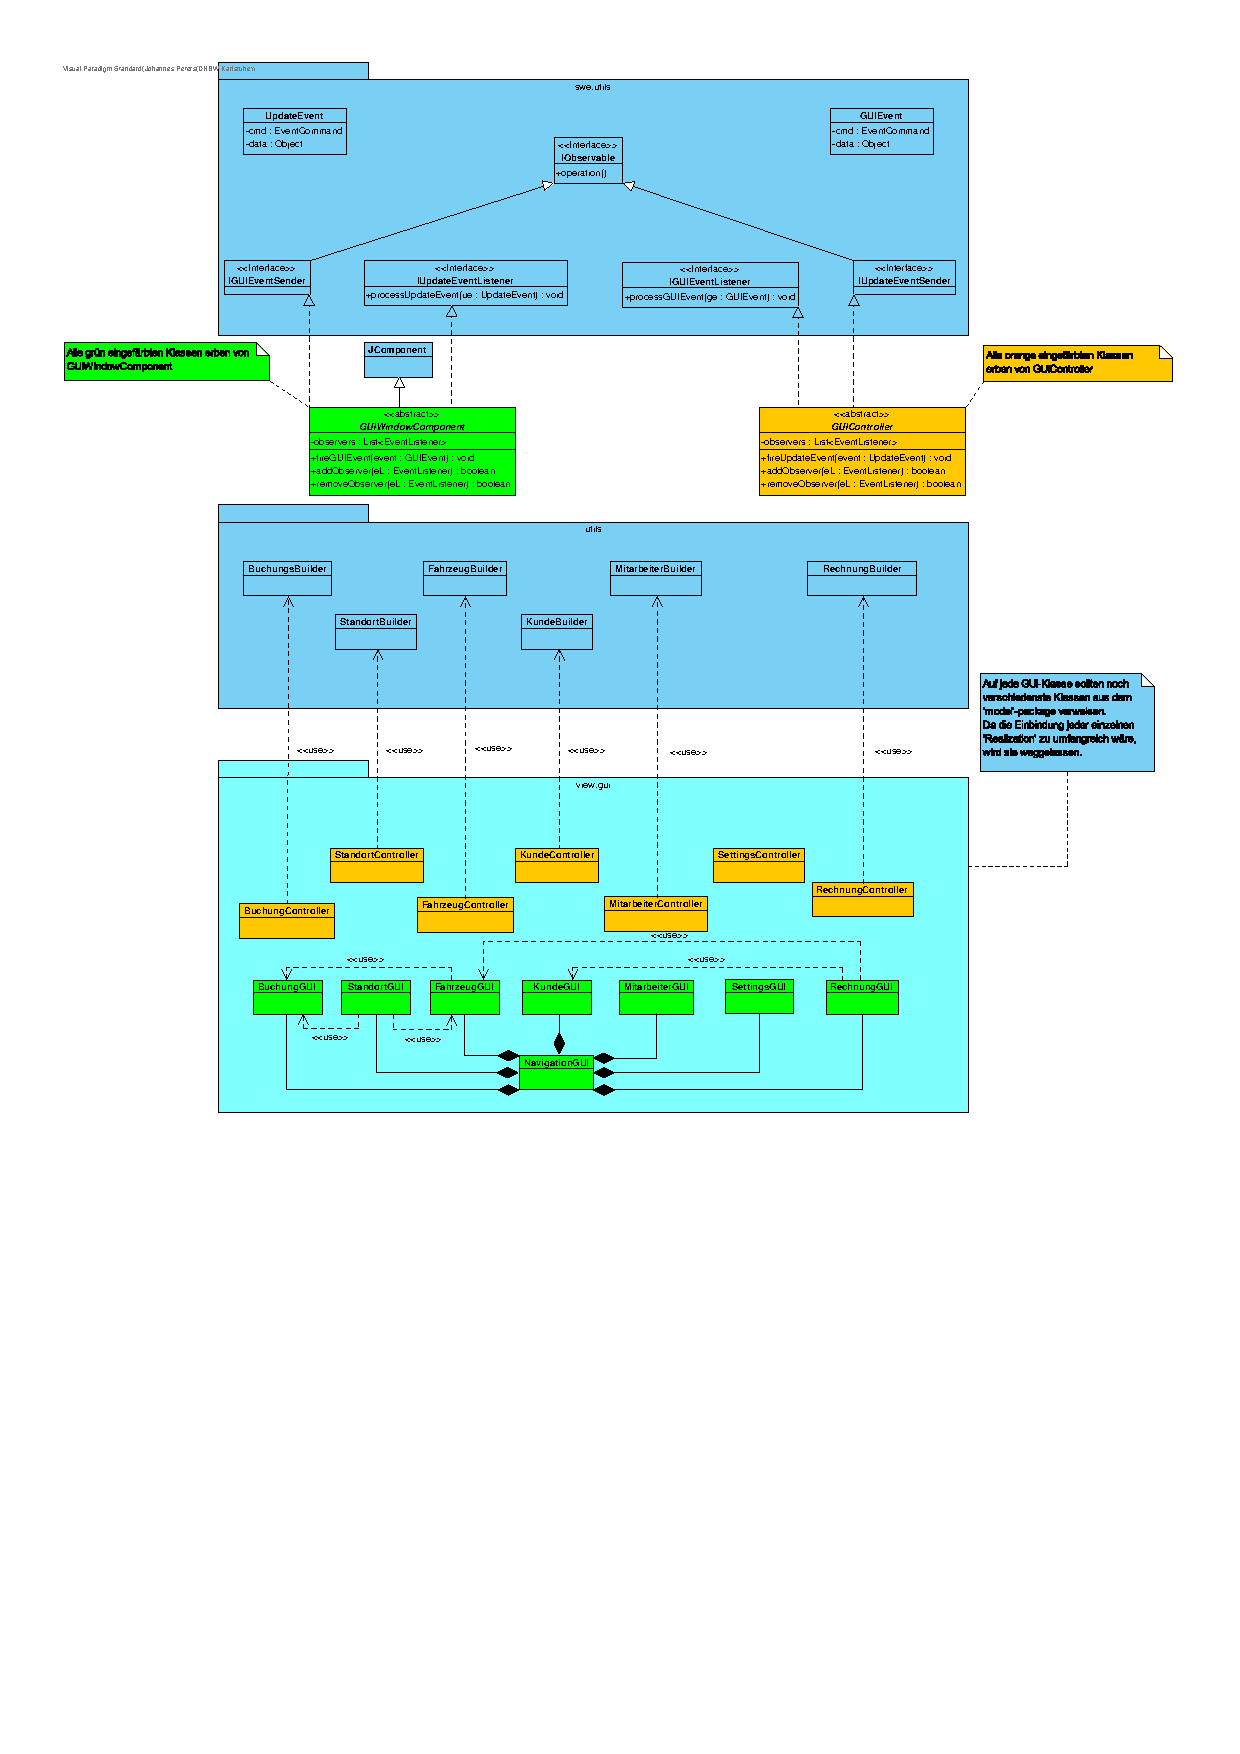
\includegraphics[width=\textwidth, trim = 0cm 10cm 0cm 0cm]{Bilder/Diagramme/EKD_GUI.pdf}
    \caption{Entwurfsklassendiagramm: GUI}
    \label{img:ekd_gui}
\end{figure}

\newpage

\section{Mock-Up}

Grundsätzlich sollen alle Verwaltungsbereiche der Anwendung den selben oder einen sehr ähnlichen Aufbau haben, damit auch Mitarbeiter ohne besondere IT-Kenntnisse die Anwendung verwenden können. Neben einer Headline, die eine Überschrift und das Firmenlogo präsentiert, gibt es an dem linken Bildschirmrand die Navigationsleiste, mit der Mitarbeiter sich durch die unterschiedlichen Verwaltungsaufgaben klicken können. Der Hauptbereich einer jeden Seite wird in zwei Felder aufgeteilt. Das linke Feld besteht aus einer Liste, in der alle Einträge zum betroffenen Verwaltungsobjekt angezeigt werden.

\subsection{Fahrzeuge verwalten}

Bei Auswahl eines Fahrzeuges erscheint im rechten Feld eine Detail-Anzeige aller nötiger Informationen, die es zu dem Listeneintrag gibt. Neben einem Filter- und Suchfeld ist natürlich auch die Manipulation der Datensätze vorgesehen, sodass man einerseits neue Fahrzeuge anlegen kann. Wie in vorhergehenden Analysen angedacht gibt es dabei einerseits einen einfachen Button mit 'anlegen' und für erfahrenere Nutzer einen Button mit '+'. Sollte ein Listeneintrag ausgewählt sein, ist auch die Bearbeitung oder das Löschen des ausgewählten Datensatzes mittels entsprechender Buttons möglich. 

\newpage

\begin{figure}[!ht]
    \centering
    \includegraphics[width=\textwidth]{Bilder/Mockup/Web 1920 – 3.png}
    \caption{Mock-Up: Liste an Fahrzeugen}
    \label{mu:fahrzeugliste}
\end{figure}

\begin{figure}[!ht]
    \centering
    \includegraphics[width=\textwidth]{Bilder/Mockup/Web 1920 – 4.png}
    \caption{Mock-Up: Detailansicht eines Fahrzeugs}
    \label{mu:fahrzeugdetails}
\end{figure}

\newpage

\textbf{Fahrzeug löschen}

Die Interaktion zum Löschen des ausgewählten Fahrzeug-Datensatzes erfolgt über ein einfaches Pop-Up-Fenster. Der Anwender muss dieses Bestätigen, wenn er den Datensatz löschen möchte, um versehentliches Löschen auszuschließen. Nach dem Löschen wird der Anwender auf die Fahrzeug-Startseite zurückverwiesen, jedoch wird in der Liste der gelöschte Eintrag entfernt. 


\begin{figure}[!ht]
    \centering
    \includegraphics[width=\textwidth]{Bilder/Mockup/Web 1920 – 5.png}
    \caption{Mock-Up: Löschen eines Fahrzeugs}
    \label{mu:loeschen}
\end{figure}

\newpage

\textbf{Fahrzeug bearbeiten}

Das Bearbeiten eines Datensatzes ist so einfach wie möglich gestaltet. Der einzige Unterschied von der Bearbeitungs-GUI zur Detail-GUI ist, dass alle Felder, die bearbeitet werden können sollen, entweder zu einem Eingabefeld oder einer Drop-Down-Liste werden. Im folgenden Beispiel werden nur die Felder 'Reifen' und 'Ausrüstung' bearbeitbar. Da es sehr unwahrscheinlich ist, dass sich bei einem bereits vorhandenen Fahrzeug der Hersteller, das Modell, die Fahrzeugklasse oder das Baujahr ändern, soll es nicht bearbeitbar sein. Informationen wie Preis, Kilometerstand werden vom System vorgegeben und einfach nur angezeigt. Es ist aber möglich bei einem Fahrzeug die Reifen zu wechseln, z.B. von Sommer- auf Winterreifen oder auch die Ausrüstung zu ändern, da z.B. eine Dachbox angebracht und wieder abmontiert werden kann. Da bei beiden Feldern keine freie Eingabe möglich sein soll, sondern nur aus Vorhandenem ausgewählt werden soll, ist die Bearbeitung mittels Checkbox-Liste vorgesehen. 


\begin{figure}[!ht]
    \centering
    \includegraphics[width=\textwidth]{Bilder/Mockup/Web 1920 – 9.png}
    \caption{Mock-Up: Bearbeiten eines Fahrzeugs}
    \label{mu:bearbeiten}
\end{figure}

\newpage

\textbf{Fahrzeug anlegen}

Die letzte ausstehende Interaktionsmöglichkeit ist das Anlegen eines neuen Fahrzeugs. Auch hier wird nur die rechte Fläche für das Erstellen verwendet. Wie beim Bearbeiten erfolgt die Eingabe über einfache Eingabefelder oder Listen. Da das Fahrzeug noch nicht angelegt wurde, hat es auch keinen Status. Informationen über Hersteller, Modell, Baujahr und Kilometerstand sind frei einzutragen, wobei es ggf. auch möglich ist Felder wie Hersteller und Baujahr als Auswahlliste zu realisieren. Die Einordnung in die Klasse erfolgt ausschließlich über eine Auswahlliste und mit Auswahl eines Eintrages wird auch der Preis des Fahrzeuges gesetzt. Reifen und Ausrüstung sind Checkbox-Listen. 

Als Vorbereitung auf die Webanwendung für Kunden und zur optisch schöneren Darstellung in der Anwendung ist es möglich ein Bild vom Fahrzeug hochzuladen. Diese Aktion ist nur für einen Admin möglich und kann jederzeit nachgeholt werden. Sollte kein Bild beim Anlegen hochgeladen werden, wird ein neutrales Platzhalter-Foto verwendet. 

\begin{figure}[!ht]
    \centering
    \includegraphics[width=\textwidth]{Bilder/Mockup/Web 1920 – 10.png}
    \caption{Mock-Up: Anlegen eines Fahrzeugs}
    \label{mu:anlegen}
\end{figure}

\subsection{Standorte verwalten}

Es ist erwünscht, dass von mindestens zwei wesentlichen GUI-Komponenten Skizzen erstellt werden. Neben der 'Verwaltung von Fahrzeugen' wird die 'Verwaltung von Standorten' genauer ausgebaut. Der Seitenaufbau ist identisch zur Fahrzeugverwaltung. Auf der Standort-Startseite befindet sich auf der linken Hälfte eine Liste mit allen eingetragenen Firmen-Standorten. Auch die zusätzlichen Interaktionsmöglichkeiten wie Suchen, Filtern und Anlegen sind identisch zu anderen Verwaltungsbereichen. Die rechte Seite der Hauptfläche wird von einer interaktiven Karte eingenommen (möglich wäre z.B. eine Einbindung von google.de/maps), auf der alle Standorte mit Markierungen eingetragen sind. 

\begin{figure}[!ht]
    \centering
    \includegraphics[width=\textwidth]{Bilder/Mockup/Web 1920 – 11.png}
    \caption{Mock-Up: Liste an Standorten}
    \label{mu:standortliste}
\end{figure}


Sofern man eine Markierung auf der Karte oder einen Listeneintrag auswählt, wird man zu einer Standort-Detail-Seite geleitet. Ebenfalls identisch vom Aufbau zur Fahrzeug-Detail-Ansicht findet man auf der rechten Seite eine detailierte Darstellung des Standortes. Dazu gehören Standortadresse, Parkplatzanzahl, das Vorhandensein von E-Ladesäulen und einer Filiale und ggf. deren Öffnungszeiten. Ebenfalls ist ein Foto angedacht. Die Fläche auf der linken Bildschirmseite ist eine Liste, doch dieses Mal werden in dieser Liste alle Fahrzeuge angezeigt, die normalerweise am Standort vorhanden sind.  

\begin{figure}[!ht]
    \centering
    \includegraphics[width=\textwidth]{Bilder/Mockup/Web 1920 – 12.png}
    \caption{Mock-Up: Detailansicht von Standorten}
    \label{mu:standortdetails}
\end{figure}

\newpage

\subsection{Buchung verwalten}

\begin{figure}[!ht]
    \centering
    \includegraphics[width=\textwidth]{Bilder/Mockup/Web 1920 – 1.png}
    \caption{Mock-Up: Listenübersicht aller Buchungen}
    \label{mu:buchung_verwalten}
\end{figure}

\begin{figure}[!ht]
    \centering
    \includegraphics[width=\textwidth]{Bilder/Mockup/Web 1920 – 2.png}
    \caption{Mock-Up: Detailansicht beim Erstellen einer Buchung}
    \label{mu:buchung_anlegen}
\end{figure}


%Der Nutzer soll die Möglichkeit haben das Design der Benutzeroberfläche auf ein 'Dark Theme' umzustellen. Durch die Auswahl des 'Dark Themes' soll die Benutzeroberfläche der Anwendung dunkler dargestellt werden. Dazu haben wir uns für folgendes Farbschema entschieden (siehe Abbildung \ref{mu:darkmode}).

%\begin{figure}[!ht]
%    \centering
%    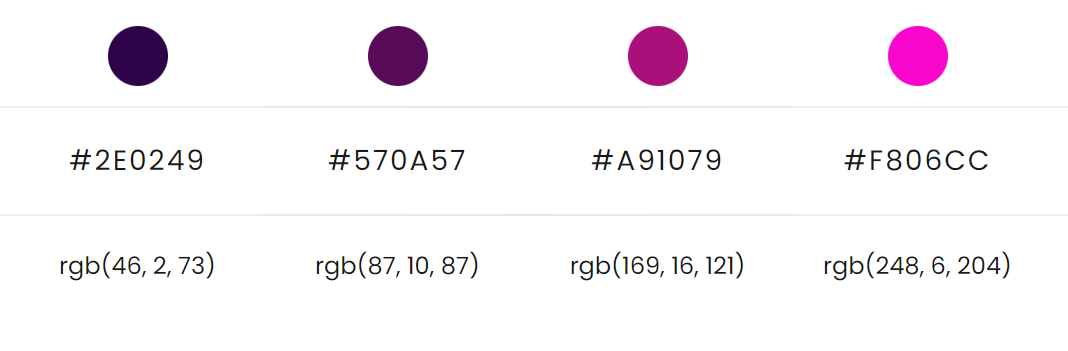
\includegraphics[width=\textwidth]{Bilder/Mockup/colorscheme_darkmode.PNG}
%    \caption{Dark Theme Farbschema}
%    \label{mu:darkmode}
%\end{figure}